\section{Weighted Least Squares (WLS)}
\subsection{Theory}
Weighted Least Squares solves a linear, overconstrained system of equations by minimizing the squared residuals of each observation equation, with a weight ($W_i$) applied to each observation.
\[
min \sum_{i}^{n} W_i\times v_i^2
\]

*Note that if the scale of the variance in the weight matrix is known to be 1, then the computed reference variance should be inspected to ensure it passes the $\chi^2$ goodness of fit test.  If it passes the test, the Covariance matrix should NOT be multiplied by the reference variance.  See definition of reference variance for the reasoning.

\subsection{Assumptions}
\begin{itemize}
	\item No Outliers/Blunders WLS is not robust to outliers (consider RANSAC/Robust Weighting if outliers)
	\item System of equations is linear (eg. derivative wrt each unknown is not a function of any of the unknowns)
	\item System is over-contrained (eg. Number of Observation Equations > Number of Unknowns)
	\item Error only in dependent variable (eg. mx+b = y + v $\rightarrow$ error only in y dimension)
	\item No covariance between weight of each observation
\end{itemize}
\subsection{Equations}
\[
WAX=WL+WV 
\]
\[
m = \text{number of observations} \hspace{1cm} 
n = \text{number of unknowns}
\]
\[
dof = \text{degrees of freedom (\# of redundant observations)} = m-n
\]
\[
A = \begin{bmatrix}
a_{11} & a_{12} & \dots & a_{1n} \\
a_{21} & a_{22} & \dots & a_{1n} \\
\vdots & \vdots & \vdots& \vdots \\
a_{m1} & a_{m2} & \dots & a_{mn} \\
\end{bmatrix}
\hspace{0.5cm}
X = 
\begin{bmatrix}
x_1 \\ x_2 \\ \vdots \\ x_n
\end{bmatrix}
\hspace{0.5cm}
L = 
\begin{bmatrix}
l_1 \\ l_2 \\ \vdots \\ l_m
\end{bmatrix}
\hspace{0.5cm}
V = 
\begin{bmatrix}
v_1 \\ v_2 \\ \vdots \\ v_m
\end{bmatrix}
\hspace{0.5cm}
W = diag\left(
\begin{bmatrix}
w_1 \\ w_2 \\ \vdots \\ w_m
\end{bmatrix}
\text{ or }
\begin{bmatrix}
\sigma^2_1 \\ \sigma^2_2 \\ \vdots \\ \sigma^2_m
\end{bmatrix}^{-1}
\right)
\]
\begin{align*}
	\text{Unknowns} &= \hat{X} = inv(A^TWA)A^TWL\\
	\text{Residuals} &= V = AX - L\\
	\text{Reference Variance} &= S_0^2 = \dfrac{V'WV}{dof} \\
	\text{Cofactor Matrix} &= Q_{xx} = inv(A^TWA) \\
	\text{Covariance Matrix of Unkowns} &= \Sigma_{xx} = S_0^2 \times Q_{xx} \\
	\text{Covariance Matrix of Observations} &= \Sigma_{\hat{l}\hat{l}} = A \Sigma_{xx} A^T \\
	\text{Standard Deviation of Solved Unknowns} &= \sigma_{\hat{X}} = \sqrt{diag(\Sigma_{xx})} \\
	\text{Predicted L} &= \hat{L} = AX \\
	\text{R$^2$ (model skill)} &= \dfrac{var(\hat{L})}{var(L)} \\
	\text{RMSE } &= \sqrt{\dfrac{VV^T}{m}} \\
\end{align*}
\clearpage
\subsection{Sample Problem}
Given the points$(x,y)$ and weights$(Weights)$: 
\[
x = [0,1,2,3,4] \hspace{1cm} y = [5,1,7,13,24] \hspace{1cm} Weights = [1,10,100,5,1]
\]
Fit a parabola given the observation equation:
\[
y = m x +b
\]
Note that the observation equation is linear, and there are no covariances to the weights.  These weights have no units, and are just saying hey, I trust the third measurement 10 times more than I trust the second measurement.
\[
A = \begin{bmatrix}
x_1 & 1 \\
x_2 & 1 \\
x_3 & 1 \\
x_4 & 1 \\
x_5 & 1 \\
\end{bmatrix} =
\begin{bmatrix}
0 & 1 \\
1 & 1 \\
2 & 1 \\
3 & 1 \\
4 & 1 \\
\end{bmatrix}
\hspace{1cm}
X = 
\begin{bmatrix}
a \\ b \\ c 
\end{bmatrix}
\hspace{1cm}
L =
\begin{bmatrix}
y_1 \\ y_2 \\ y_3 \\ y_4 \\ y_5
\end{bmatrix} = 
\begin{bmatrix}
5 \\ 1 \\ 7 \\ 13 \\ 24
\end{bmatrix}
\hspace{1cm}
W = 
\begin{bmatrix}
15 & 0 & 0 & 0 & 0 \\
0 & 10 & 0 & 0 & 0 \\
0 & 0 & 100 & 0 & 0 \\
0 & 0 & 0 & 5 & 0 \\
0 & 0 & 0 & 0 & 1 \\
\end{bmatrix}
\]
Use the Equations and solve:
\begin{table}[H]
\centering
\begin{tabular}{|c|c|c|}
\toprule
$n = 3$& %NEWCOLUMN
$m = 5$& %NEWCOLUMN
$dof = 2$\\ %NEWROW
\midrule
$\hat{X} = $$
 \begin{bmatrix}
1.33\\
0.52\\
0.52\\
\end{bmatrix}
$
& %NEWCOLUMN
$V = $ $
 \begin{bmatrix}
-4.48\\
1.36\\
-0.14\\
1.01\\
-0.19\\
\end{bmatrix}
$
& %NEWCOLUMN
$S_0^2 = 22.88$ \\ %NEWROW
\midrule
$\Sigma_{xx} = $ $
 \begin{bmatrix}
0.55&-2.09&1.89\\
-2.09&9.01&-9.21\\
1.89&-9.21&10.59\\
\end{bmatrix}
$
& %NEWCOLUMN
$\sigma_{\hat{X}} = $ $
 \begin{bmatrix}
0.74\\
3.00\\
3.25\\
\end{bmatrix}
$
& %NEWCOLUMN
$\Sigma_{\hat{l}\hat{l}} = $ $
 \begin{bmatrix}
10.59&3.28&-0.25&0.02&4.07\\
3.28&1.34&0.09&-0.46&-0.32\\
-0.25&0.09&0.22&0.14&-0.15\\
0.02&-0.46&0.14&1.82&4.59\\
4.07&-0.32&-0.15&4.59&13.88\\
\end{bmatrix}
$
\\ %NEWROW
\midrule
$Q_{xx} = $ $
 \begin{bmatrix}
0.02&-0.09&0.08\\
-0.09&0.39&-0.40\\
0.08&-0.40&0.46\\
\end{bmatrix}
$
& %NEWCOLUMN
$\hat{L} = $$
 \begin{bmatrix}
0.52\\
2.36\\
6.86\\
14.01\\
23.81\\
\end{bmatrix}
$
& %NEWCOLUMN
$R^2 = 1.1366$ \hspace{1cm} $RMSE = 2.15$\\ %NEWROW
\bottomrule
\end{tabular}
\end{table}


\begin{figure}[H]
	\centering
	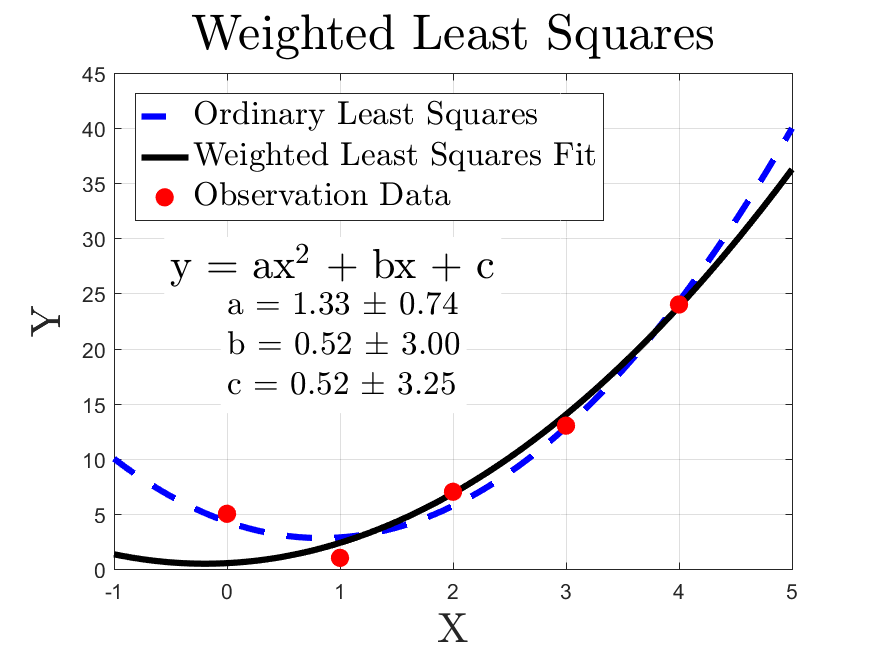
\includegraphics[height = 3.25in]{WLSexample.png}
\end{figure}

\subsection{Example Matlab Code}
\lstinputlisting[
label      = {alg:exampleWLS},
caption    = {exampleWLS.m},
style      = Matlab-editor,
basicstyle = \mlttfamily,
firstline  = 1,
lastline   = 25,
firstnumber= 1
]{exampleWLS.m}

\lstinputlisting[
label      = {alg:exampleWLS2},
caption    = {The Matlab built in function LSCOV generates the same results},
style      = Matlab-editor,
basicstyle = \mlttfamily,
firstline  = 27,
lastline   = 28,
firstnumber= 25
]{exampleWLS.m}

